\section{Materials and methods}\label{sec:methods}

\subsection{Data}\label{sec:data}


The multi-parametric \ac{mri} data are acquired from a cohort of patients with higher-than-normal level of \ac{psa}.
The acquisition is performed using a 3T whole body \ac{mri} scanner (Siemens Magnetom Trio TIM, Erlangen, Germany) using sequences to obtain \ac{t2w}-\ac{mri}, \ac{dce}-\ac{mri} and \ac{dw}-\ac{mri}.
Aside of the \ac{mri} examination, these patients also have underwent a guided-biopsy.
The dataset is composed of a total of 20 patients of which 18 patients have biopsy proven \ac{cap} and 2 patients are ``healthy'' with negative biopsies.
Therefore, 13 patients have a \ac{cap} in the \ac{pz}, 3 patients have \ac{cap} in the \ac{cg}, 2 patients have invasive \ac{cap} in both \ac{pz} and \ac{cg} and finally 2 patients are considered as ``healthy''.
An experienced radiologist has segmented the prostate organ --- on \ac{t2w}-\ac{mri} and \ac{dce}-\ac{mri} --- as well as the prostate zones (i.e., \ac{pz} and \ac{cg}) and \ac{cap} on the \ac{t2w}-\ac{mri}.

A \SI{3}{\mm} slice fat-suppressed \ac{t2w} fast spin-echo sequence (\ac{tr}/\ac{te}/\ac{etl}: \SI{3400}{\ms}/\SI{85}{\ms}/13) is used to acquire images in sagittal and oblique coronal planes, the latter planes being orientated perpendicular or parallel to the prostate \ac{pz} – rectal wall axis.
Three-dimensional \ac{t2w} fast spin-echo (\ac{tr}/\ac{te}/\ac{etl}: \SI{3600}{\ms}/\SI{143}{\ms}/109, slice thickness: \SI{1.25}{\mm}) images are then acquired in an oblique axial plane.
The nominal matrix and \ac{fov} of the 3D \ac{t2w} fast spin-echo images are $320 \times 256$ and $280 \times 240$ mm\textsuperscript{2}, respectively, thereby affording sub-millimetric pixel resolution within the imaging plane.

\ac{dce}-\ac{mri} are performed using a fat suppressed 3D T1 VIBE sequence (\ac{tr}/\ac{te}/Flip angle: \SI{3.25}{\ms}/\SI{1.12}{\ms}/\SI{10}{\degree}; Matrix: $256 \times 192$; \ac{fov}: $280 \times 210$ (with 75\% rectangular \ac{fov}); slab of 16 partitions of \SI{3.5}{\mm} thickness; temporal resolution: \SI{6}{\s}/slab over approximately \SI{5}{\minute}).
A power injector (Medrad, Indianola, USA) is used to provide a bolus injection of Gd-DTPA (Dotarem, Guerbet, Roissy, France) at a dose of \SI{0.2}{\ml} Gd-DTPA/kg of body weight.

These \ac{dce}-\ac{mri} sequences are resampled using the spatial information of the \ac{t2w}-\ac{mri} and missing data are interpolated using linear interpolation.
The volumes of the \ac{dce}-\ac{mri} dynamic are rigidly registered, to remove any patient motion during the acquisition.
Furthermore, a non-rigid registration is performed between the \ac{t2w}-\ac{mri} and \ac{dce}-\ac{mri} in order to propagate the prostate zones and \ac{cap} ground-truths.
The resampling is implemented in C++ using the Insight Segmentation and Registration Toolkit~\citep{ibanez2005itk}.

\subsection{Implementation}

The implementation of the registration (C++), normalization (Python), and classification pipeline (Python) are publicly available on GitHub\footnote{\url{https://github.com/I2Cvb/lemaitre-2016-nov/tree/master}}.
The data used for this work are also publicly available\footnote{\url{http://kaggle.com}}.

\subsection{Normalization of \ac{dce}-\ac{mri} images}\label{sec:norm}

\begin{figure}
  \centering
  \hspace*{\fill}
  \subfigure[Patient 1]{\label{subfig:pat1}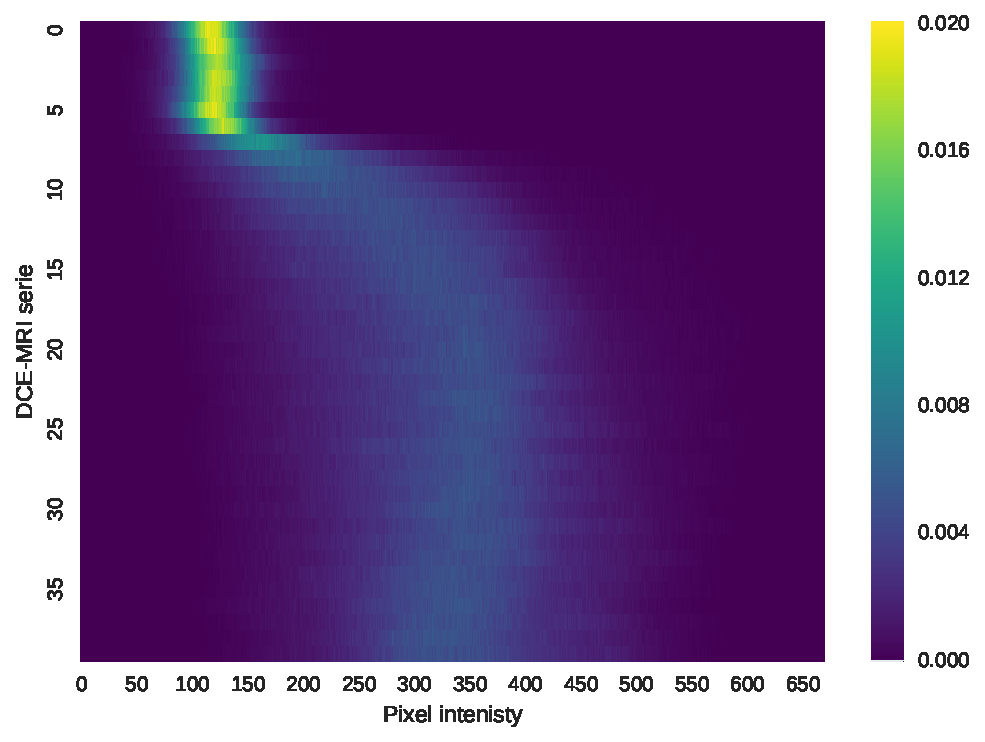
\includegraphics[width=.49\textwidth]{02_methods/figures/pat1.pdf}} \hfill
  \subfigure[Patient 2]{\label{subfig:pat2}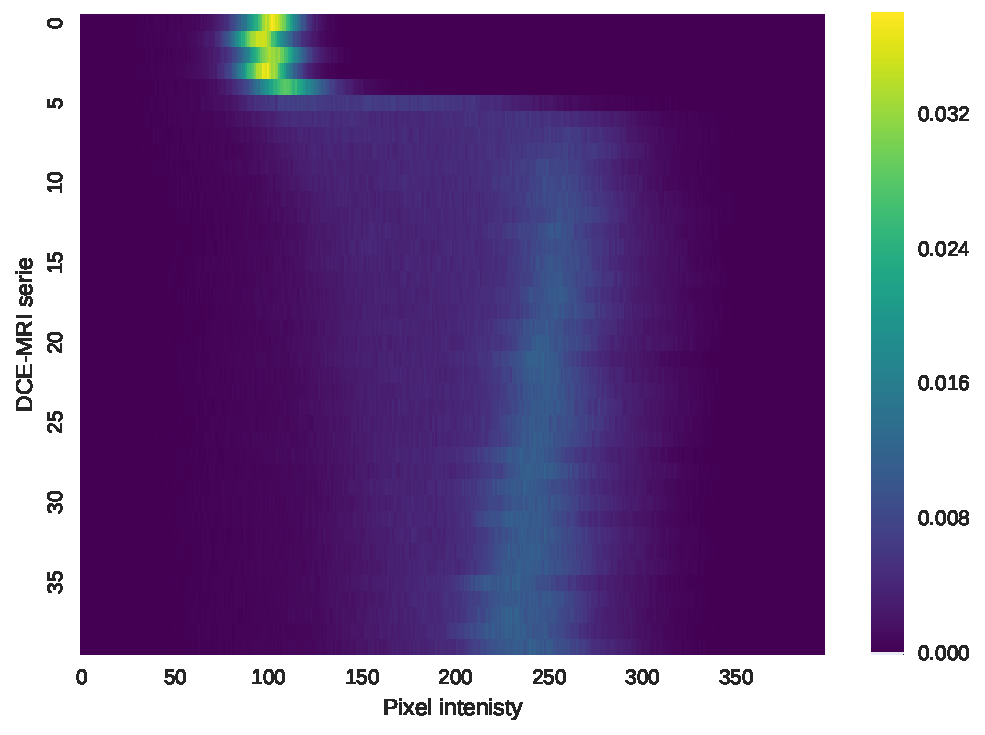
\includegraphics[width=.49\textwidth]{02_methods/figures/pat2.pdf}}
  \hspace*{\fill}
  \caption{Illustration of the variations of the intensity \acs*{pdf} over time of two patients in a \ac{dce}-\ac{mri}.}
  \label{fig:heatmap}
\end{figure}

In this work, we propose a method to normalize \ac{dce}-\ac{mri} prostate data, although it can be applied to any \ac{dce}-\ac{mri} sequences.
The aim of the method is to reduce the intra-patient variations, occuring during the acquisition process.
In \ac{t2w}-\ac{mri}, these variations imply that the intensity \ac{pdf} of the prostate region is shifted as well as wider or narrower, from a patient to another.
Therefore, these variations can be corrected using a $z$-score approach, assuming that the data follow a specific distribution~\citep{lemaitre2016normalization}.

In \ac{dce}-\ac{mri}, the inter-patient variations are more complex due to the over time acquisition.
These variations can be highlighted by observing the evolution of the intensity \ac{pdf} of the \ac{dce}-\ac{mri} over time, as shown in the heatmap in Fig.\,\ref{fig:heatmap}.
Therefore, these variations are:
(i) an offset of the peak value before pre-contrast,
(ii) a time offset depending of the contrast injection, and
(iii) a global scale factor related to the enhancement.
Therefore, our normalization method should attenuate all these variations and be performed globally across the different time sequence rather than for each independent sequence.

\subsubsection{Graph-based offset correction for each \ac{dce}-\ac{mri} sequence}

\begin{figure}
  \centering
  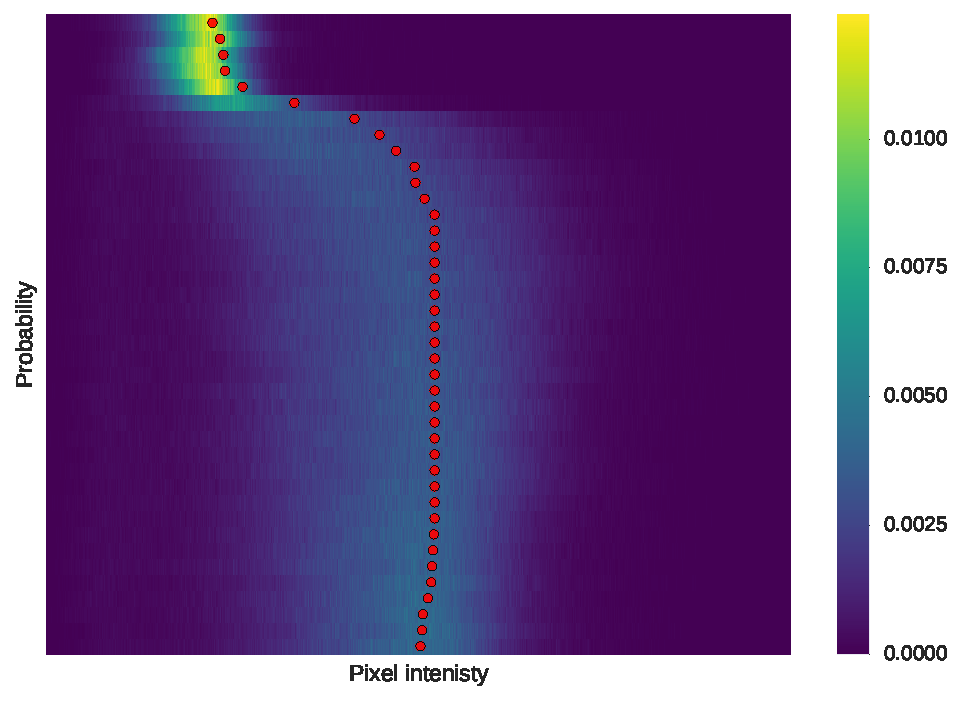
\includegraphics[width=0.7\linewidth]{02_methods/figures/estimator.pdf}
  \caption{Illustration of the estimator found using the shortest-path through the graph.}
  \label{fig:estimator}
\end{figure}

Before to standardize each sequence, the first step of the normalization is to cancel the intensity shift which is specific for each patient.
The intensity \ac{pdf} do not follow either a Rician or Gaussian distribution over time.
Therefore, the mean cannot be used as a potential estimate for the offset.
Additionally, this offset should be characterized by a smooth transition over time.
This problem can be solved using the graph-theory: considering the intensity \ac{pdf} over time as shown in Fig.\,\ref{fig:heatmap}, the offset is the boundary splitting the heatmap in two partitions such that it is as close as possible to the peak of the intensity \ac{pdf} (see Fig.\,\ref{fig:estimator} for an illustration).
Given the heatmap, a directed weighted graph $\mathcal{G}=(\mathcal{V}, \mathcal{E})$ is built by taking each bar of the heatmap as a node and connecting each pair of bars by an edge.
The edge weight $w_{ij}$ between two nodes $i$ and $j$ corresponding to two pixels at position $(x_i, y_i)$ and $(x_j, y_j)$, respectively, is defined as in Eq.\,\eqref{eq:weight}:

\begin{equation}
  w_{ij} = \begin{cases}
    \alpha \exp(1 - \frac{H(i)}{\max(H)})       & \text{if } x_j = x_i + 1 \text{ and } y_j = y_i \\
    (1 - \alpha) \exp(1 - \frac{H(i)}{\max(H)}) & \text{if } x_j = x_i \text{ and } y_j = y_i + 1 \\
    0                                           & \text{otherwise}
  \end{cases} ,
  \label{eq:weight}
\end{equation}

\noindent where $H$ is the heatmap, $\alpha$ is a smoothing parameter controlling the partitioning.

Therefore, the offset is estimated by finding the shortest-path to cross the graph using Dijkstra algorithm.
The entry and exiting nodes are set to be the bin with the maximum probability for the first \ac{dce}-\ac{mri} serie and the bin corresponding to the median value for the last \ac{dce}-\ac{mri} serie, respectively.
To ensure a robust estimation of the offset, the process of finding the shortest-path is iteratively repeated by shifting the data and updating the heatmap as well as the graph $\mathcal{G}$.
The procedure is stopped once that the offset found do not change.
In general, this process is not repeated more than 3 iterations.
An example of the offset found using this approach is presented in Fig.\,\ref{fig:estimator}.
Finally, each sequence is shifted using this offset.

\subsubsection{Time offset and data dispersion correction}

\begin{figure}
  \centering
  \hspace*{\fill}
  \subfigure[\acs*{rmse} computed for each patient of our dataset.]{\label{fig:rmse}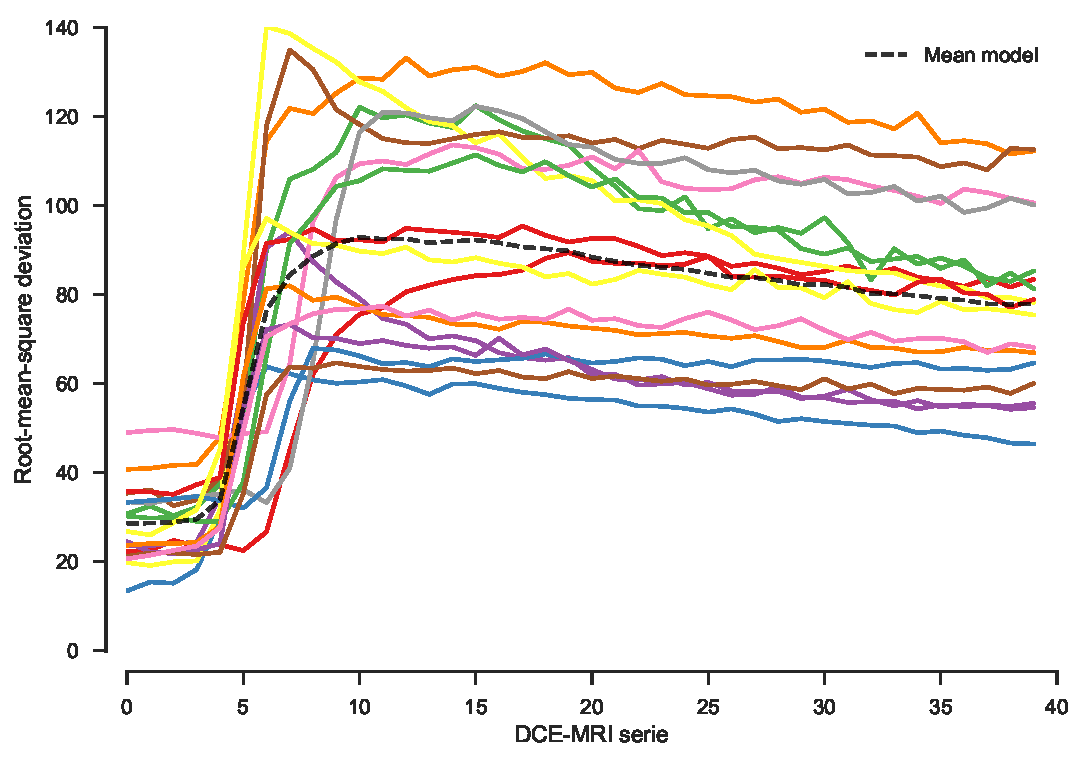
\includegraphics[width=.49\textwidth]{02_methods/figures/rmse.pdf}} \hfill
  \subfigure[\acs*{rmse} after alignment using the curve parametric model.]{\label{fig:rmseal}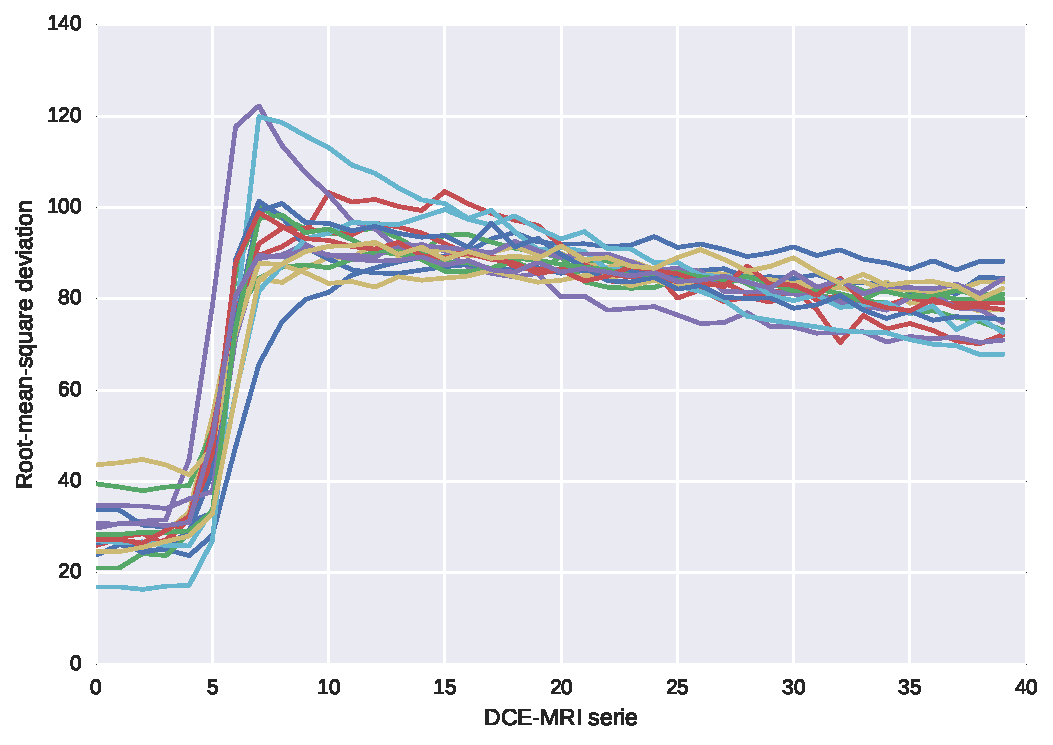
\includegraphics[width=.49\textwidth]{02_methods/figures/rmse_aligned.pdf}}
  \hspace*{\fill}
  \caption{Illustration of the correction of the time offset and the data dispersion.}
  \label{fig:curveal}
\end{figure}

The next variations to correct are the time offset and the data dispersion.
By computing the \ac{rmse} for each \ac{dce}-\ac{mri}, one can observed these two variations as shown in Fig.\,\ref{fig:rmse}.
Therefore, to correct these variations, we propose to register each patient \ac{rmse} to a mean model which corresponds to the mean of all patients \ac{rmse}.
The parametric model to perform the registration is formulated as in Eq.\,\eqref{eq:model}:

\begin{equation}
  T(\alpha, \tau, f(t)) = \alpha f(t - \tau) ,
  \label{eq:model}
\end{equation}

\noindent where $\alpha$ and $\tau$ are the two parameters handling the time offset and global scale, respectively, $f(\cdot)$ is the \ac{rmse} function.

Therefore the registration problem is equivalent to:

\begin{equation}
  \argmin_{\alpha, \tau} = \sum_{t=0}^{N} \left[ T\left(\alpha, \tau, f(t)\right) - \mu(t) \right]^{2} ,
  \label{eq:cost}
\end{equation}

\noindent where $\mu(\cdot)$ is the mean model, $N$ is the number of \ac{dce}-\ac{mri} serie.

Illustration of the correction applied to each \ac{rmse} patient is shown in Fig.\,\ref{fig:rmseal}.
Once all these parameters have been inferred, the data can be shifted as well as scale.

\subsection{Quantification of \ac{dce}-\ac{mri}}\label{sec:stateart}

\subsubsection{Brix and Hoffmann models}\label{sec:brixhoffmann}

In the Brix model~\citep{brix1991pharmacokinetic}, the \ac{mri} signal intensity is assumed to be proportional to the media concentration.
Therefore, the model is expressed as in Eq.\,\eqref{eq:brix}:

\begin{equation}
  s_n(t) = 1 + A \left[ \frac{\exp(k_{el} t') - 1}{k_{ep}(k_{ep} - k_{el})} \exp(- k_{el} t) - \frac{\exp(k_{ep} t') - 1}{k_{el}(k_{ep} - k_{el})} \exp(- k_{ep} t) \right],
  \label{eq:brix}
\end{equation}

\noindent with

\begin{equation}
  s_n(t) = \frac{s(t)}{S_0},
  \label{eq:enh}
\end{equation}

\noindent where $s(t)$ and $S_0$ are the \ac{mri} signal intensity at time $t$ and the average pre-contrast \ac{mri} signal intensity, respectively; $A$, $k_{el}$, and $k_{ep}$ are a constant proportional to the transfer constant, the diffusion rate constant, and the rate constant, respectively. Additionally, during the injection time $0 \leq t \leq \tau$, $t' = t$ and afterwards while $t > \tau$, $t' = \tau$.

Following this model, \citeauthor{hoffmann1995pharmacokinetic} propose the following similar model as expressed in Eq.\,\eqref{eq:hoffmann}:

\begin{equation}
  s_n(t) = 1 + \frac{A}{\tau} \left[ \frac{k_{ep} \left( \exp(k_{el} t') - 1 \right)}{k_{el}(k_{ep} - k_{el})} \exp(- k_{el} t) - \frac{\exp(k_{ep} t') - 1}{(k_{ep} - k_{el})} \exp(- k_{ep} t) \right].
  \label{eq:hoffmann}
\end{equation}

The parameters are estimated by fitting the model using non-linear least-squares optimization solved with Levenberg-Marcquardt.

\subsubsection{Tofts model}\label{sec:tofts}

The extended Tofts model is formulated as in Eq.\,\eqref{eq:exttofts}:

\begin{equation}
  C_t(t) = K_{trans} C_p(t) \Conv \exp(-k_{ep}t) + v_p C_p(t),
  \label{eq:exttofts}
\end{equation}

\noindent where $\Conv$ is the convolution operator; $C_t(t)$ and $C_p(t)$ is the concentration of contrast agent in the tissue and in the plasma, respectively; $K_{trans}$, $k_{ep}$, and $v_p$ are the volume transfer constant, the diffusion rate constant, and the plasma volume fraction, respectively.

Therefore, Tofts model requires to:
(i) detect candidate voxels from the femoral or iliac arteries and estimate a patient-based \ac{aif} signal,
(ii) convert the \ac{mri} signal intensity (i.e., \ac{aif} and dynamic signal) to a concentration, and
(iii) in the case of a population-based \ac{aif}, estimate an \ac{aif} signal.

\begin{figure}
  \centering
  \hspace*{\fill}
  \subfigure[Original image.]{\label{fig:org}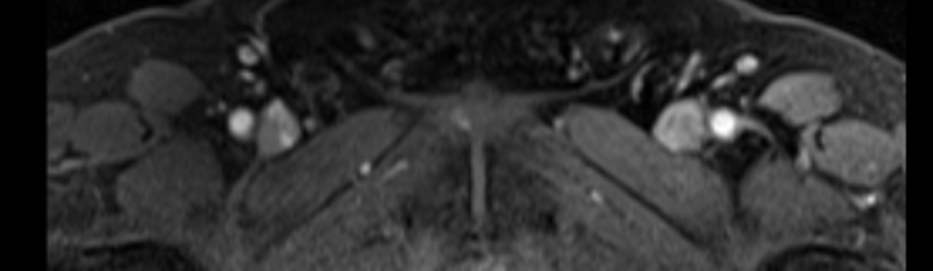
\includegraphics[width=.3\textwidth]{02_methods/figures/original.pdf}} \hfill
  \subfigure[Candidates region after clustering.]{\label{fig:cand}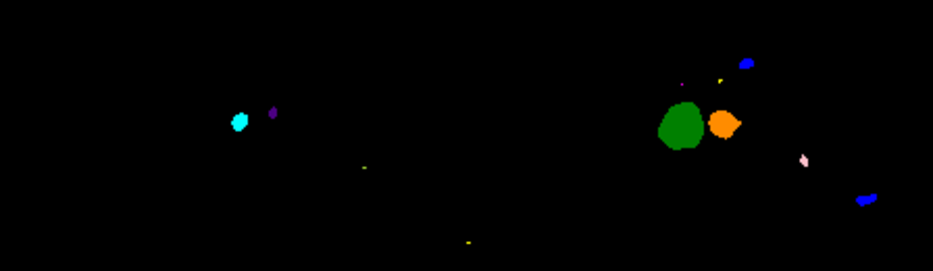
\includegraphics[width=.3\textwidth]{02_methods/figures/candidate.pdf}} \hfill
  \subfigure[Regions selected after applying the different criteria.]{\label{fig:final}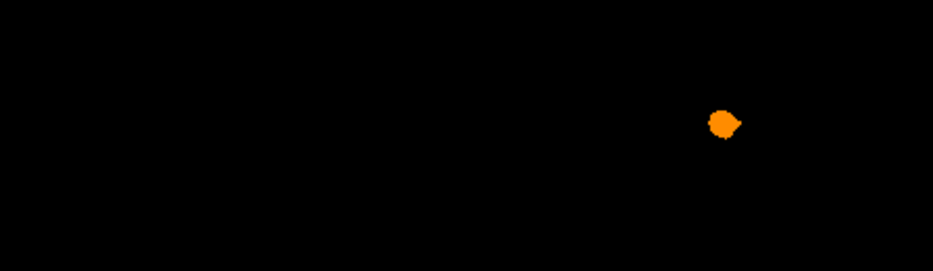
\includegraphics[width=.3\textwidth]{02_methods/figures/aif.pdf}}
  \hspace*{\fill}
  \caption{Illustration of the segmentation of the area used to determine the \acs*{aif}.}
  \label{fig:aif}
\end{figure}

\begin{description}
  \item[Segmentation of artery voxels and patient-based \ac{aif} estimation] The \ac{aif} signal from \ac{dce}-\ac{mri} can be manually estimated by selecting the most-enhanced voxels from the femoral or iliac arteries~\citep{meng2010comparison}.
    Few methods have been proposed to address the automated extraction of \ac{aif} signal.
    \citeauthor{chen2008automatic} filter successively the possible candidates~\citep{chen2008automatic}:
    (i) dynamic signals with small peak are rejecting by thresholding,
    (ii) voxels with a small wash-in are rejected by thresholding,
    (iii) a blob detector is used and large enough regions are kept, and
    (iv) circular and cylindricality are used to reject the last false positive.
    \citeauthor{zhu2011automated} propose an iterative method selecting voxels which best fit a gamma variate function~\citep{zhu2011automated}.
    However, it requires to compute first and second derivatives as well as maximum curvature points.
    \citeauthor{shanbhag2012generalized} propose a 4-steps algorithm~\citep{shanbhag2012generalized,fennessy2015quantitative}:
    (i) remove slices with artefacts and find the best slices based on intrinsic anatomic landmarks and enhancement characteristics,
    (ii) find the voxel candidates using the maximum enhanced voxels and a multi-label maximum entropy based thresholding algorithm,
    (iii) excluding region next to the endorectal coil, and
    (iv) selecting the best 5 candidates which meet enhancement characteristics and that are correlated.

    All the above methods are rather complex and thus we propose a method which is based on the following simple assumptions:
    (i) all possible \ac{aif} signal candidates should have a similar shape,
    (ii) an high enhancement, and
    (iii) the arteries should be almost round and within a size range.
    Therefore, each slice is clustered into regions using K-means clustering with $k=6$.
    The cluster with the highest enhancement\textemdash i.e. corresponding to the 90\textsuperscript{th} percentile of the maximum of each dynamic signal\textemdash contain the arteries and is selected.
    Finally, regions with an eccentricity smaller than $0.5$ and an area in the range of $[100, 400]$ voxels are kept.
    Additionally, to remove voxels contaminated by partial volume effect, only the $10\%$ most enhanced voxels of the possible candidates are kept as proposed by~\citep{schabel2008uncertainty} and the average signal is computed.
    A summary of the different segmentation steps is presented in Fig.\,\ref{fig:aif}.
    \item[Conversion of \ac{mri} signal intensity to concentration] To estimate the free parameters of the Tofts model (see Eq.\,\eqref{eq:exttofts}), the concentration $C_t(t)$ and $C_p(t)$ need to be computed from the \ac{mri} signal intensity and the \ac{aif} signal, respectively.
      This conversion is based on the equation of the FLASH sequence\textemdash see~\ref{app:signaltoconc} for details\textemdash and is formulated as in Eq.\,\eqref{eq:conv}:
      \begin{equation}
        c(t) = \frac{1}{TR \cdot r_1} \ln\left( \frac{1 - \cos \alpha \cdot S^{*}\frac{s(t)}{S_0}}{1 - S^{*}\frac{s(t)}{S_0}} \right) - \frac{R_{10}}{r_1} ,
        \label{eq:conv}
      \end{equation}
      \noindent with,
      \begin{equation}
        S^{*} = \frac{1 - \exp(- TR \cdot R_{10})}{1 - \cos \alpha \cdot \exp(- TR \cdot R_{10})} ,
        \label{eq:sstarconv}
      \end{equation}
      \noindent where $s(t)$ is the \ac{mri} signal, $S_0$ is the \ac{mri} signal prior to the injection of the contrast media, $\alpha$ is the flip angle, $TR$ is the \acf{tr}, $R_{10}$ is the pre-contrast tissue relaxation time also equal to $\frac{1}{T_{10}}$, $r_1$ is the relaxitivity coefficient of the contrast agent.

      $T_{10}$ can be estimated from the acquisition of a T$_1$ map.
      However, this modality was not part of the clinical trial in this research and the value of $T_{10}$ was fixed to \SI{1600}{\ms} for both blood and prostate as stated in the literature~\citep{fennessy2015quantitative,de2004mr,carr2011magnetic}.
      \item[Estimation of population-based \ac{aif}] While estimating the pharmacokinetic parameters from Tofts model, the \ac{aif} concentration $C_p(t)$ can be computed either from the patient or a population.
        We presented in the two previous sections the algorithms which allows to estimate the patient-based \ac{aif} concentration.
        To compare with the previous approach, we also computed a population-based \ac{aif} which will be also later used to compare the performance of both approaches.
        In that regard, the population-based \ac{aif} was estimated as in~\citep{meng2010comparison} by fitting the average patient-based \ac{aif}s to the model of~\cite{parker2006experimentally} which is formulated as in Eq.\,\eqref{eq:parker}:
        \begin{equation}
          C_p(t) = \sum_{n=1}^{2} \frac{A_n}{\sigma_n \sqrt{2 \pi}} \exp\left(\frac{- (t- T_n)^2}{2\sigma_{n}^{2}}\right) + \frac{\alpha \exp(-\beta t)}{1 + \exp{-s (t - \tau)}} ,
          \label{eq:parker}
        \end{equation}
        \noindent where $A_n$, $T_n$, and $\sigma_n$ are the scaling constants, centers, and widths of the n\textsuperscript{th} Gaussian, $\alpha$ and $\beta$ are the amplitude and decay constant of the exponential; and $s$ and $\tau$ are the width and center of the sigmoid function, respectively.
\end{description}

The parameters are estimated by fitting the model using non-linear least-squares optimization solved with Levenberg-Marcquardt.

\subsubsection{\acs*{pun} model}\label{sec:pun}

\citeauthor{gliozzi2011phenomenological} show that \ac{pun} approach can be used for \ac{dce}-\ac{mri} analysis~\citep{gliozzi2011phenomenological}.
The model has been successfully used in a \ac{cad} system proposed by~\cite{giannini2015fully}.
This model can be expressed as in Eq.\,\eqref{eq:pun}:

\begin{equation}
  s_n(t) = \exp\left[rt + \frac{1}{\beta} \left( a_0 - r \right) \left( \exp(\beta t) - 1 \right) \right],
  \label{eq:pun}
\end{equation}

\noindent with

\begin{equation}
  s_n(t) = \frac{s(t) - S_0}{S_0},
  \label{eq:enh}
\end{equation}

\noindent where $s(t)$ and $S_0$ are the \ac{mri} signal intensity at time $t$ and the average pre-contrast \ac{mri} signal intensity, respectively; $r$, $a_0$, and $\beta$ are the free parameters of the model.

The parameters are estimated by fitting the model using non-linear least-squares optimization solved with Levenberg-Marcquardt.

\subsubsection{Semi-quantitative analysis}\label{sec:semi}

The semi-quantitative analysis of the \ac{dce}-\ac{mri} is equivalent to extract curve characteristics directly from the signal without a strict theoretical pharmacokinetic meaning.
In this work, we use the model presented by~\cite{huisman2001accurate} which formulate the \ac{mri} signal as in Eq.\,\eqref{eq:huisman}:

\begin{equation}
  s(t) = \begin{cases}
    S_0 & 0 \leq t \leq t_0 \\
    S_M - (S_M - S_0) \exp\left( \frac{-(t - t_0)}{\tau} \right) & t_0 < t \leq t_0 + 2 \tau \\
    S_M - (S_M - S_0) \exp\left( \frac{-(t - t_0)}{\tau} \right) + w(t - t_0 + 2 \tau) & t > t_0 + 2 \tau
  \end{cases}
  \label{eq:huisman}
\end{equation}

\noindent where $s(t)$ is the \ac{mri} signal intensity, $S_0$ is the pre-contrast signal intensity, $t_0$ is the time corresponding to the start of enhancement, $S_M$ and $\tau$ is the maximum of the signal and the exponential time constant, and $w$ is the slope of the linear part.

\citeauthor{huisman2001accurate} argue that curve fitting via least-squares minimization using Nelder-Mead algorithm leads to inaccurate estimation of the free parameters: mainly the issue come from an incorrect estimation of the start of enhancement $t_0$ leading to incorrect estimation of the other parameters.
Therefore, they propose to:
(i) estimate robustly $t_0$,
(ii) estimate $S_0$ by averaging the samples between $0$ and $t_0$
(ii) estimate $w$ depending if the slope is significant or not,
(iii) estimate $S_M$ which should be the point at the intersection of the most probable slope line and the plateau.

Instead of these successive estimations, we propose a unified optimization in which $t_0$ is fixed since that this is a key parameter.
Therefore, $t_0$ is robustly estimated from the \ac{aif} signal since that this is the most enhanced signal in which the start of enhancement is easily identifiable.
The \ac{aif} signal is computed as in Section~\ref{sec:tofts}.
$t_0$ is estimated by finding the maximum in the beginning of the first derivative of the \ac{mri} signal.
Then, the function in Eq.\,\eqref{eq:huisman} is fitted using non-linear least squares with Trust Region Reflective algorithm.
Furthermore, the parameters $\tau$ and $S_M$ are bounded during the optimization to ensure robust estimations.

From Eq.\,\eqref{eq:huisman}, the following features are extracted:
(i) the wash-in corresponding to the slope between $t_0$ and $t_0 + 2 \tau$,
(ii) the wash-out corresponding to the parameter $w$,
(iii) the area under the curve between $t_0$ and the end of the signal,
(iv) the exponential time constant $\tau$, and
(v) the relative enhancement $S_M - S_0$.

%%% Local Variables: 
%%% mode: latex
%%% TeX-master: "../main"
%%% End: 
